\documentclass[10pt,landscape,a4paper]{article}

\usepackage[utf8]{inputenc}
\usepackage{amsfonts}

\usepackage{mathtools}
\usepackage{enumitem}

%\usepackage[ngerman]{babel}
%\usepackage[T1]{fontenc}
%\usepackage[nosf]{kpfonts}
%\usepackage[t1]{sourcesanspro}
\usepackage[dvipsnames]{xcolor}
\usepackage{tikz}
\usetikzlibrary{shapes,positioning,arrows,fit,calc,graphs,graphs.standard}
\usepackage{multicol}
\usepackage{wrapfig}
\usepackage[top=0mm,bottom=1mm,left=0mm,right=1mm]{geometry}
\usepackage[framemethod=tikz]{mdframed}
\usepackage{microtype}
\usepackage{pdfpages}
\usepackage{verbatim}

\let\bar\overline
\let\ul\underline
\let\del\partial

\definecolor{myblue}{cmyk}{1,.72,0,.38}



\def\firstcircle{(0,0) circle (1.5cm)}
\def\secondcircle{(0:2cm) circle (1.5cm)}

\colorlet{circle edge}{myblue}
\colorlet{circle area}{myblue!5}

\tikzset{filled/.style={fill=circle area, draw=circle edge, thick},
    outline/.style={draw=circle edge, thick}}


%Own Operators----------------------------------------------------------------------------------------------------------------------------------------------------------------------------------------------------
\DeclareMathOperator*{\argmax}{arg\,max}
\DeclareMathOperator*{\argmin}{arg\,min}
\DeclareMathOperator*{\curl}{curl}

\let\div\relax %remove the existing div command to allow operator definition
\DeclareMathOperator*{\div}{div}

\DeclareMathOperator*{\grad}{grad}



%Own Commands----------------------------------------------------------------------------------------------------------------------------------------------------------------------------------------------------
%1. Inequality in set: ieset
%Default: lhs is tau
\newcommand{\ieset}[2][\tau]{\{#1 \le #2\}} 
%Example: to get {X <= t} use this expression $\ieset[X]{t}$

%2. Conditional Expectation for Sigma Algebra: scEx
%Default: sigma Algebra is F_n
\newcommand{\scEx}[2][n]{E[#2 \mid \mathfrak{F}_#1]}
%Example: to get E[ X | F_tau ] use this expression $\scEx[\tau]{X}$

%3. In curly brackets: icb
\newcommand{\icb}[1]{\{ #1 \}}
%Example: to get {a = b} use this expression $\icb{a = b}

%4. Norm: norm
\newcommand{\norm}[1]{\left\lVert#1\right\rVert}
%Example: to get ||X|| use the expression \norm{X}

%5. Column Vector
\newcommand*\colvec[1]{\begin{pmatrix}#1\end{pmatrix}}
%Example: \colvec{a \\ b} gives vector (a,b) transposed.

%6.Row Vector
\newcommand{\rvec}[1]{\begin{bmatrix} #1 \end{bmatrix}}
%Example: \rvect{a & b} gives vector (a,b)




\pgfdeclarelayer{background}
\pgfsetlayers{background,main}


\everymath\expandafter{\the\everymath \color{myblue}}


\renewcommand{\baselinestretch}{.8}
\pagestyle{empty}


\global\mdfdefinestyle{header}{%
linecolor=gray,linewidth=1pt,%
leftmargin=0mm,rightmargin=0mm,skipbelow=0mm,skipabove=0mm,
}


\newcommand{\header}{
\begin{mdframed}[style=header]
\footnotesize
\sffamily
Cheat Sheet\\
Page \thepage
\end{mdframed}
}


\makeatletter % Author: https://tex.stackexchange.com/questions/218587/how-to-set-one-header-for-each-page-using-multicols
\renewcommand{\section}{\@startsection{section}{1}{0mm}%
                                {.2ex}%
                                {.2ex}%x
                                {\color{myblue}\sffamily\small\bfseries}}
\renewcommand{\subsection}{\@startsection{subsection}{1}{0mm}%
                                {.2ex}%
                                {.2ex}%x
                                {\sffamily\bfseries}}




\makeatother
\setlength{\parindent}{0pt}






\begin{document}
%\footnotesize
%\small
\begin{multicols*}{4}
\section{Vector Calculus}

\subsection*{Scalar Fields}
$f : \mathbb{R}^n \to \mathbb{R}$

\subsection*{Vector Fields}
$\ul{v} : \mathbb{R}^n \to \mathbb{R}^m$

\subsection*{Differentiation of Vector Fields}
Let $\ul{a}, \ul{b}, \ul{c}$ be vector fields and $\varphi$ be a scalar field, then
\[
\begin{aligned}
	\frac{d}{dt} (\varphi \ul{a})= & \frac{d\varphi}{dt}  \ul{a}+ \varphi \frac{d\ul{a}}{dt}\\
	\frac{d}{dt} (\ul{a} \cdot \ul{b})= &  \frac{d\ul{a}}{dt} \cdot \ul{b} +  \ul{a} \cdot \frac{d\ul{b}}{dt}\\
	\frac{d}{dt} (\ul{a} \times \ul{b})= &  \frac{d\ul{a}}{dt} \times \ul{b} +  \ul{a} \times \frac{d\ul{b}}{dt} \\
	\frac{d}{dt} ( \ul{a}(\varphi(t) ) )= & \frac{d\ul{a}}{d\varphi} \frac{d\varphi}{dt} \\
\end{aligned}
\]

\subsection*{Differential Operators}
For a scalar field $f : \mathbb{R}^n \to \mathbb{R}, \ul{x} \mapsto f(\ul{x})$ the gradient is
\[
	\grad f(\ul{x})  = \colvec{ \frac{\del f}{\del x_1} \\ \vdots \\ \frac{\del f}{\del x_n} } 
\]
and gives the direction of \ul{steepest ascent}


For a vector field $\ul{v} : \mathbb{R}^n \to \mathbb{R}^n$ the divergence is defined as 
\[
	\div \ul{v}(\ul{x}) = \sum_{j=1}^n \frac{\del v_j}{\del x_j}(\ul{x})
\]
and gives the \ul{source density} at a point

For a vector field $\ul{v} : \mathbb{R}^3 \to \mathbb{R}^3$ the curl is defined as 
\[
	\curl(\ul{v}(x,y,z)) = \colvec{ \frac{\del v_3}{\del y} - \frac{\del v_2}{\del z} \\
						 \frac{\del v_1}{\del z} - \frac{\del v_3}{\del x}  \\
						 \frac{\del v_2}{\del x}  - \frac{\del v_1}{\del y} }
\]
and gives the \ul{vortex strength}


The Laplace operator for a scalar field $f : \mathbb{R}^n \to \mathbb{R}, \ul{x} \mapsto f(\ul{x})$ gives
\[
	\Delta f(\ul{x})  = \nabla \cdot \nabla f(\ul{x}) = \sum_{j=1}^n \frac{\del^2 f}{\del^2 x_j}(\ul{x})
\]


Expressed with the $\nabla$ operator we get the representations
\[
 \begin{aligned}
	\grad f = & \nabla f \\
	\div \ul{v} = & \nabla \cdot \ul{v}\\
	\curl \ul{v} = &  \nabla \times \ul{v} \\
	\Delta = & \nabla \cdot \nabla \\
\end{aligned}
\]

\subsection*{Computation Rules for Differential Operators}
The three operators grad, div and curl are linear. 
Rules for one active operator:
\[
\begin{aligned}
	\grad (f_1 f_2) =& f_1 \, \grad f_2 + f_2 \, \grad f_1\\
	\Leftrightarrow \nabla (f_1 f_2) = & f_1 \, \nabla  f_2 + f_2 \, \nabla f_1\\
	\\
	\grad F(f) =& F'(f) \, \grad f \\
	\Leftrightarrow \nabla F(f) = & F'(f) \, \nabla f \\
	\\
	\div (\ul{v}_1 \times \ul{v}_2) =& \ul{v}_2 \cdot \curl \ul{v}_1 - \ul{v}_1 \cdot \curl \ul{v}_2 \\
	\Leftrightarrow \nabla \cdot (\ul{v}_1 \times \ul{v}_2) = &  \ul{v}_2 \cdot (\nabla \times \ul{v}_1) - \ul{v}_1 \cdot (\nabla \times \ul{v}_2) \\
\end{aligned}
\]

Rules for the interactions between vector- and scalarfields:
\[
\begin{aligned}
	\div f \ul{v} = &  \ul{v} \, \grad f + f \div \ul{v}\\
	\Leftrightarrow \nabla \cdot (f\ul{v}) = &  \ul{v} \, \nabla f + f (\nabla \cdot \ul{v})\\
	\\
	\curl f \ul{v} = &  f \curl \ul{v}  -  \ul{v} \times \grad f\\
	\Leftrightarrow \nabla \times (f \ul{v}) = &  f (\nabla \times\ul{v})  -  \ul{v} \times \nabla f\\
\end{aligned}
\]


Rules for the concatenation of the operators:
\[
\begin{aligned}
	\div \curl \ul{v} = &  0 \\
	\Leftrightarrow \nabla \cdot ( \nabla \times\ul{v} ) = &  0 \\
	\\
	\curl \grad f = &  \ul{0} \\
	\Leftrightarrow \nabla \times \nabla f = & \ul{0}\\
	\\
	\div \grad f = & \Delta f \\
	\Leftrightarrow \nabla \cdot \nabla f = &  \Delta f\\
	\\
	\curl \curl \ul{v} = & \grad  \div \ul{v} - \Delta \ul{v} \\
	\Leftrightarrow \nabla \times (\nabla \times \ul{v}) =  & \nabla  (\nabla \cdot \ul{v}) - \Delta \ul{v}\\
\end{aligned}
\]



\subsection*{Flux ($\Phi$)}

\textbf{Q}: Let be $\ul{v}$ the velocity field of a flow;
how much fluid flows through a surface $S$ per unit time in direction $\ul{n}$?

\textbf{A}: Split $S$ into infinitesimal area elements $dS$. 
Because they are infinitesimal, the $dS$ are flat and $\ul{v}$ is homogeneous within a single $dS$.
The total flow through a single $dS$ is
\[
	d\Phi = \ul{v} \cdot \ul{n} dS
\]

The flux is the “sum” over all infinitesimal $dS$ and thus given by the integral
\[
	\Phi = \int_S \ul{v} \cdot \ul{n} dS
\]






\begin{comment}
\subsection*{Exercise}

\[
\begin{aligned}
& \text { curl curl }=\text { curl }\left(\begin{array}{l}
\frac{\partial}{\partial y} v_3-\frac{\partial}{\partial z} v_2 \\
\frac{\partial}{\partial z} v_1-\frac{\partial}{\partial x} v_3 \\
\frac{\partial}{\partial x} v_2-\frac{\partial}{\partial y} v_1
\end{array}\right) \\
& =\left(\begin{array}{l}
\frac{\partial}{\partial x} \\
\frac{\partial}{\partial y} \\
\frac{\partial}{\partial z}
\end{array}\right) \times\left(\begin{array}{l}
\frac{\partial}{\partial y} v_3-\frac{\partial}{\partial z} v_2 \\
\frac{\partial}{\partial z} v_1-\frac{\partial}{\partial x} v_3 \\
\frac{\partial}{\partial x} v_2-\frac{\partial}{\partial y} v_1
\end{array}\right) \\
& \left.=\left(\begin{array}{l}
\left(\frac{\partial^2}{\partial x \partial y} v_2-\frac{\partial^2}{\partial y^2} v_1\right)-\left(\frac{\partial^2}{\partial z^2} v_1-\frac{\partial^2}{\partial x \partial z} v_3\right. \\
\left.\frac{\partial^2}{\partial z \partial y} v_3-\frac{\partial^2}{\partial z^2} v_2\right)-\left(\frac{\partial^2}{\partial x^2} v_2-\frac{\partial^2}{\partial x \partial y} v_1\right. \\
\left.\frac{\partial^2}{\partial x \partial z} v_1-\frac{\partial^2}{\partial x^2} v_3\right)-\left(\frac{\partial^2}{\partial y^2} v_3-\frac{\partial^2}{\partial y \partial z} v_2\right.
\end{array}\right)\right) \\
& =\left(\begin{array}{l}
\frac{\partial^2}{\partial x \partial y_2} v_2+\frac{\partial^2}{\partial x \partial z} v_3-\frac{\partial^2}{\partial y^2} v_1-\frac{\partial^2}{\partial z^2} v_1+\frac{\partial^2}{\partial x \partial x} v_1-\frac{\partial^2}{\partial x^2} v_1 \\
\frac{\partial^2}{\partial z \partial y^2} v_3+\frac{\partial^2}{\partial x \partial y} v_1-\frac{\partial^2}{\partial y^2} v_2-\frac{\partial^2}{\partial \partial^2} v_2+\frac{\partial^2}{\partial y \partial y} v_2-\frac{\partial^2}{\partial y^2} v_2 \\
\frac{\partial^2}{\partial x \partial z} v_1+\frac{\partial^2}{\partial y \partial z} v_2-\frac{\partial^2}{\partial y^2} v_3-\frac{\partial^2}{\partial z^2} v_3+\frac{\partial^2 y}{\partial z \partial z} v_3-\frac{\partial^2}{\partial z^2} v_3
\end{array}\right) \\
& =\left(\begin{array}{l}
\frac{\partial^2}{\partial x \partial y} v_2+\frac{\partial^2}{\partial x \partial z} v_3+\frac{\partial^2}{\partial x^2} v_1-\Delta v_1 \\
\frac{\partial^2}{\partial z \partial \partial v_3}+\frac{\partial^2}{\partial x \partial y} v_1+\frac{\partial^2}{\partial y^2} v_2-\Delta v_2 \\
\frac{\partial^2}{\partial x \partial z} v_1+\frac{\partial^2}{\partial y \partial z} v_2+\frac{\partial^2}{\partial z^2} v_3-\Delta v_3
\end{array}\right) \\
& =\left(\begin{array}{c}
\frac{\partial}{\partial x}\left(\frac{\partial}{\partial x} v_1+\frac{\partial}{\partial y} v_2+\frac{\partial}{\partial z} v_3\right) \\
\frac{\partial}{\partial y}\left(\frac{\partial}{\partial x} v_1+\frac{\partial}{\partial y} v_2+\frac{\partial}{\partial z} v_3\right) \\
\frac{\partial}{\partial z}\left(\frac{\partial}{\partial x} v_1+\frac{\partial}{\partial y} v_2+\frac{\partial}{\partial z} v_3\right)
\end{array}\right)-\Delta \mathbf{v} \\
& =\left(\begin{array}{l}
\frac{\partial}{\partial x} \\
\frac{\partial}{\partial y} \\
\frac{\partial}{\partial z}
\end{array}\right)\left(\frac{\partial}{\partial x} v_1+\frac{\partial}{\partial y} v_2+\frac{\partial}{\partial z} v_3\right)-\Delta \mathbf{v} \\
& =\operatorname{grad} d i v \mathbf{v}-\Delta \mathbf{v} \\
&
\end{aligned}
\]

\begin{comment}













\begin{comment}


\begin{aligned}
	\grad(f_1 f_2) = & f_1 \grad( f_2) + f_2 \grad(f_1 )\\
	\gradF(f) = & F'(f) \grad(f) \\
	\div f\ul{v} = &  \ul{v} \grad( f) + f \div \ul{v}\\
	\div \ul{v} = & \nabla \cdot \ul{v}\\
	\curl \ul{v}_1 + \ul{v}_2 = &  \curl \ul{v}_1 + \curl \ul{v}_2\\
	\curl c\ul{v} = &  c \curl \ul{v} \\
	\curl f \ul{v} = &  f \curl\ul{v}  -  \ul{v} \times \grad(f)\\
	\div\curl \ul{v} = &  0 \\
	\curl\grad f = &  \ul{0} \\
	\div\grad f = & \Delta f \\
	\curl\curl \ul{v} = & \grad  \div \ul{v} - \Delta \ul{v} \\
	\div (\ul{v}_1 \times \ul{v}_2) = & \ul{v}_2 \cdot \curl\ul{v}_1 - \ul{v}_1 \cdot \curl\ul{v}_2 \\
\end{aligned}


1. Wenn $F \wedge G$ eine Tautologie ist, dann ist $F$ eine Tautologie und $G$ auch.
2. Umgekehrt: Sind $F$ und $G$ Tautologien, dann ist auch $F \wedge G$ eine.
\emph{Beweis.}
1. Annahme: $F \wedge G$ sei eine Tautologie.
Dann: Für jede Belegung $B$ wertet $F \wedge G$ zu wahr aus.
Dann: Das ist nur der Fall, wenn sowohl $F$ als auch $G$ (für jedes $B$) zu wahr auswerten.
Dann: Für jede Belegung $B$ wertet $F$ zu wahr aus. Und:
Für jede Belegung $B$ wertet $G$ zu wahr aus.
Dann: $F$ ist Tautologie und $G$ ist Tautologie.
2. Annahme: $F$ ist Tautologie und $G$ ist Tautologie.
Dann: Für jede Belegung $B_1$ wertet $F$ zu wahr aus. Und: Für jede Belegung $B_2$ wertet $G$ zu wahr aus.
Dann: Für jede Belegung $B$ wertet $F \wedge G$ zu wahr aus.
Dann: $F \wedge G$ ist eine Tautologie.
\subsection*{Äquivalenz und Folgerung}
$p\equiv q$ gilt genau dann, wenn sowohl $p\models q$ als auch $q\models p$ gelten. \emph{Beweis.}
$p\equiv q$ GDW $p\Leftrightarrow q$ ist Tautologie nach Def. von $\equiv$
GDW $(p\Rightarrow q) \wedge (q\Rightarrow p)$ ist Tautologie
GDW $(p\Rightarrow q)$ ist Tautologie und $(q\Rightarrow p)$ ist Tautologie
GDW $(p\models q)$ gilt und $q\models p$ gilt.
\subsection*{Substitution}
Ersetzt man in einer Formel eine beliebige Teilformel $F$ durch eine logisch äquivalente
Teilformel $F'$, so verändert sich der Wahrheitswerteverlauf der Gesamtformel nicht.
Man kann Formeln also vereinfachen, indem man Teilformeln durch äquivalente
(einfachere) Teilformeln ersetzt.
\subsection*{Universum}
Die freien Variablen in einer Aussagenform können durch Objekte aus einer als
Universum bezeichneten Gesamtheit wie $\mathbb{N},\mathbb{R},\mathbb{Z},\mathbb{Q}$ ersetzt werden.
\subsection*{Tautologien}
$(p\wedge q)\Rightarrow p$\text{ bzw. }$p\Rightarrow (p\vee q)$\\
$(q\Rightarrow p)\vee (\neg q\Rightarrow p)$\\
$(p\Rightarrow q)\Leftrightarrow (\neg p\vee q)$\\
$(p\Rightarrow q)\Leftrightarrow (\neg q\Rightarrow\neg p)$ \hfill\text{(Kontraposition)}\\
$(p\wedge (p\Rightarrow q))\Rightarrow q$ \hfill\text{(Modus Ponens)}\\
$((p\Rightarrow q)\wedge (q\Rightarrow r))\Rightarrow (p\Rightarrow r)$\\
$((p\Rightarrow q)\wedge (p\Rightarrow r))\Rightarrow (p\Rightarrow (q\wedge r))$\\
$((p\Rightarrow q)\wedge (q\Rightarrow p))\Leftrightarrow (p\Leftrightarrow q)$
\subsection*{Nützliche Äquivalenzen}
Kommutativität:\\
$(p \wedge q) \equiv (q \wedge p)$\\
$(p \vee q) \equiv (q \vee p)$\\
Assoziativität:\\
$(p \wedge (q \wedge r)) \equiv ((p \wedge q) \wedge r)$\\
$(p \vee (q \vee r)) \equiv ((p \vee q) \vee r)$\\
Distributivität:\\
$(p \wedge (q \vee r)) \equiv ((p \wedge q) \vee (p \wedge r))$\\
$(p \vee (q \wedge r)) \equiv ((p \vee q) \wedge (p \vee r))$\\
Idempotenz:\\
$(p \wedge p) \equiv p$\\
$(p \vee p) \equiv p$\\
Doppelnegation:\\
$\neg (\neg p) \equiv p$\\
de Morgans Regeln:\\
$\neg (p \wedge q) \equiv ((\neg p) \vee (\neg q))$\\
$\neg (p \vee q) \equiv ((\neg p) \wedge (\neg q))$\\
Definition Implikation:\\
$(p \Rightarrow q) \equiv (\neg p \vee q)$\\
Tautologieregeln:\\
$(p \wedge q) \equiv p$\hfill (falls $q$ eine Tautologie ist)\\
$(p \vee q) \equiv q$\\
Kontradiktionsregeln:\\
$(p \wedge q) \equiv q$\hfill (falls $q$ eine Kontradiktion ist)\\
$(p \vee q) \equiv p$\\
Absorptionsregeln:\\
$(p \wedge (p \vee q)) \equiv p$\\
$(p \vee (p \wedge q)) \equiv p$\\
Prinzip vom ausgeschlossenen Dritten:\\
$p \vee (\neg p) \equiv w$\\\
Prinzip vom ausgeschlossenen Widerspruch:\\
$p \wedge (\neg p) \equiv f$
\subsection*{Äquivalenzen von quant. Aussagen}
Negationsregeln:\\
$\neg\forall x:p(x)\equiv\exists x:(\neg p(x))$\\
$\neg\exists x:p(x)\equiv\forall x:(\neg p(x))$\\
Ausklammerregeln:\\
$(\forall x:p(x)\wedge\forall y:q(y))\equiv\forall z:(p(z)\wedge q(z))$\\
$(\exists x:p(x)\wedge\exists y:q(y))\equiv\exists z:(p(z)\wedge q(z))$\\
Vertauschungsregeln\\
$\forall x\forall y:p(x,y)\equiv\forall y\forall x:p(x,y)$\\
$\exists x\exists y:p(x,y)\equiv\forall y\exists x:p(x,y)$
\subsection*{Äquivalenzumformung}
Wir demonstrieren an der Formel $\neg (\neg p \wedge q) \wedge (p \vee q)$, wie man mit Hilfe der
aufgelisteten logischen Äquivalenzen tatsächlich zu Vereinfachungen kommen kann:\\
$\phantom{{}\equiv{}} \neg (\neg p \wedge q) \wedge (p \vee q)$\\
$\equiv (\neg (\neg p) \vee (\neg q)) \wedge (p \vee q)$\hfill de Morgan\\
$\equiv (p \vee (\neg q)) \wedge (p \vee q)$\hfill Doppelnegation\\
$\equiv p \vee ((\neg q) \wedge q)$\hfill Distributivtät v.r.n.l.\\
$\equiv p \vee (q \wedge (\neg q))$\hfill Kommutativtät\\
$\equiv p \vee f$\hfill Prinzip v. ausgeschl. Widerspruch\\
$\equiv p$\hfill Kontradiktionsregel

\end{comment}




\section{Modeling Spatial Effects}

\subsection*{Reynolds transport theorem}

\begin{align*}
 \frac{D \varphi}{D t} & =\frac{D}{D t} \int_{V(t)} f d V(t) \\
& =\int_{V(t)} \frac{D f}{D t} d V(t)+\int_{V(t)} f \underbrace{\frac{D}{D t}[d V(t)]}_{
	%\partial d V(t) 
	\underbrace{\frac{\partial d V(t)}{\partial t}}_{= 0}
	+(\ul{v} \cdot \nabla) d V(t) 
 }\\
& =\int_{V(t)}\left[\frac{D f}{D t}+f(\ul{v} \cdot \nabla)\right] d V(t) \\
& =\int_{V(t)}[\frac{\partial f}{\partial t}+\underbrace{\ul{v} \cdot(\nabla f)+f(\nabla \cdot \ul{v})}_{
	=\nabla \cdot(f \ul{v}): \text { see compute rules }}] d V(t) \\
& =\int_{V(t)}\left[\frac{\partial f}{\partial t}+\nabla \cdot(f \ul{v})\right] d V(t) \text {. } \\
\end{align*}


\subsection*{Vector Fields}
$\ul{v} : \mathbb{R}^n \to \mathbb{R}^m$




%\section{Relationen}
\subsection*{Binäre Relation}
Eine binäre Relation $R$ ist eine Menge von Paaren $(a,b)\in A\times B$.\\
$aRb\Leftrightarrow (a,b)\in R$ bzw. $a(\neg R)b\Leftrightarrow (a,b)\notin R$\\
\emph{Beispiele:}\\
Teilerrelation ($nTm$): $P_3:=\{(n,m+3)\mid n,m\in\mathbb{N}\}=\{(1,4),(2,5),(3,6),...\}$\\
Relation $\subset$ über $\mathcal{P}(M)$ für $M=\{1,2\}$:\\
$\{(\emptyset ,\{1\}),(\emptyset ,\{2\}),(\emptyset ,\{1,2\}),(\{1\},\{1,2\}),\\(\{2\} ,\{1,2\})\}$
\subsection*{Inverse Relation}
Sei $R\subseteq A\times B$. Die inverse Relation zu $R$ ist $R^{-1}=\{(y,x)\in B\times A\mid (x,y)\in R\}$. Also ist $R^{-1}\subseteq B\times A$.\\
\emph{Beispiel:} Sei $R=\{(1,a),(1,c),(3,b)\}$ dann ist $R^{-1}=\{(a,1),(c,1),(b,3)\}$
\subsection*{Komposition}
Seien $R\subseteq M_1\times M_2$ und $S\subseteq M_2\times M_3$ zweistellige Relationen.
Die Verknüpfung $(R\circ S)\subseteq (M_1\times M_3)$ heißt Komposition der Relationen $R,S$.\\
$R\circ S:=\{(x,z)\mid\exists y\in M_2:(x,y)\in R\wedge (y,z)\in S\}$\\
\emph{Beispiel:} Sei $R=\{(1,2),(2,5),(5,1)\}$, dann ist $R^2=R\circ R=\{(1,5),(2,1),(5,2)\}$\\
Sei $R\subseteq\mathbb{N}\times\mathbb{N}$ mit $(n,m)\in R\Leftrightarrow m=3n$ und
$S\subseteq\mathbb{N}\times\mathbb{Z}$ mit $(n,z)\in S\Leftrightarrow z=-n$. Dann ist $R\circ S=\{(n,z)\mid z=-3n\}\subseteq\mathbb{N}\times\mathbb{Z}$
\subsection*{Eigenschaften von Operationen}
$(R\cup S)^{-1}=R^{-1}\cup S^{-1}$\\
$(R\cap S)^{-1}=R^{-1}\cap S^{-1}$\\
$(R\circ S)^{-1}=S^{-1}\circ R^{-1}$\\
$(R\cap S)\circ T\subseteq (R\circ T)\cap (S\circ T)$\\
$T\circ (R\cap S)\subseteq (T\circ R)\cap (T\circ S)$\\
$(R\cup S)\circ T = (R\circ T)\cup (S\circ T)$\\
$T\circ (R\cup S) = (T\circ R)\cup (T\circ S)$
\subsection*{Eigenschaften von Relationen}
Reflexiv: $\forall a\in A:(a,a)\in R$\\
Symmetrisch: $\forall a,b\in A:(a,b)\in R\Rightarrow (b,a)\in R$\\
Antisymm.: $\forall a,b\in A:(a,b)\in R\wedge (b,a)\in R\Rightarrow a=b$\\
Transitiv: $\forall a,b,c\in A:(a,b)\in R\wedge (b,c)\in R\Rightarrow (a,c)\in R$\\
Total: $\forall a,b \in A: (a,b)\in R\vee (b,a)\in R$\\
Irreflexiv: $\forall a\in A: (a,a)\notin R$\\
Asymm.: $\forall a,b\in A:(a,b)\in R\Rightarrow (b,a)\notin R$\\
Alternativ: $\forall a,b\in A:(a,b)\in R\oplus (b,a)\in R$\\
Rechtseind.: $\forall a\in A:(a,b)\in R\wedge (a,c)\in R\Rightarrow b=c$\\
Linkseind.: $\forall a\in A:(b,a)\in R\wedge (c,a)\in R\Rightarrow b=c$\\
Eindeutig: $R$ ist recht- und linkseindeutig.\\
Linkstotal: $\forall a\in A\exists b\in B:(a,b)\in R$\\
Rechtstotal: $\forall b\in B\exists a\in A:(a,b)\in R$
\subsection*{Äquivalenzrelation}
Ist eine Relation $\sim$ reflexiv, symmetrisch und transitiv, heißt sie Äquivalenzrelation.
\subsection*{Äquivalenzklassen}
Gegeben eine Äquivalenzrelation $R$ über der Menge $A$.
Dann ist für $a\in A$: $[a]_R=\{x\mid (a,x)\in R\}$ die Äquivalenzklasse von $a$.\\
(Äquivalente Elemente kommen in die gleiche Menge)\\
\emph{Beispiel (Restklassen):}\\
$[4]=\{n\mid n\mod 3=4 \mod 3\}=[1]$\\
$[5]=\{n\mid n\mod 3=5 \mod 3\}=[2]$\\
$[6]=\{n\mid n\mod 3=6 \mod 3\}=[3]$
\subsection*{Zerlegungen, Partition}
Eine Zerlegung (Partition) $\mathcal{Z}$ ist eine Einteilung von $A$ in nicht leere, paarweise
elementfremde Teilmengen, deren Vereinigung mit $A$ übereinstimmt.\\
\emph{Beispiel:} Sei $A=\{1,2,3,...,10\}$. Dann ist $\mathcal{Z_1}=\{\{1,3\},\{2,5,9\},\{4,10\},\{6,7,8\}\}$
\subsection*{Abschluss einer Relation}
$R_\phi^*$ bildet die fehlenden Relationen mit der Eigenschaft $\phi$, also alle Kombinationen aus $A$, die noch nicht in $R$ sind.\\
\emph{Beispiel:}\\
Sei $A=\{1,2,3\}$ und $R=\{(1,2),(2,3),(3,3)\}$. 
Dann ist $R_{refl}^*=R\cup\{(1,1),(2,2)\}$,\\
$R_{sym}^*=R\cup\{(2,1),(3,2)\}$,
$R_{tra}^*=R\cup\{(1,3)\}$
\subsection*{Halbordunung}
Eine Relation $R$, die reflexiv, antisymmetrisch und transitiv ist.
%\section{Abbildungen}
Eine Abbildung $f:X\to Y$ ist eine Vorschrift, die jedem $x\in X$ eindeutig ein bestimmtes
$y=f(x)\in Y$ zuordnet. $y$ ist das \emph{Bild} von $x$ und $x$ das \emph{Urbild} von $y$.
Für eine Abbildung gilt, dass jedes Element der Urmenge $X$ genau auf ein $y\in Y$ abbildet, es müssen aber nicht alle Elemente aus $Y$ angenommen werden bzw. darf auch mehrfach angenommen werden (rechtseindeutig, linksvollständig).\\
Als Relation:\\
$f\subseteq A\times B$ mit $f=\{(a,f(a))\mid a\in A\wedge f(a)\in B\}$
\subsection*{Funktionen}
Sei $f\subseteq A\times B$ linkseindeutige und rechtsvollständige Relation.\\
$F$ ist linksvollständig, wenn gilt $\forall a\in A\exists b\in B:(a,b)\in R$.\\
$F$ ist rechtseindeutig, wenn gilt $\forall a\in A\forall b_1,b_2\in B:(a,b_1)\in R\wedge
(a,b_2)\in R\Rightarrow b_1=b_2$.
\subsection*{Bild, Urbild}
Sei $f:A\to B$ und $M\subseteq A$.\\
Das \emph{Bild} von $M$ unter $f$ ist die Menge $f(M):=\{f(x)\mid x\in M\}$.\\
Das \emph{Urbild} einer Teilmenge $N\subseteq B$ heißt $f^{-1}(N):=\{a\in A\mid f(a)\in N\}$.
\subsection*{Eigenschaften von Abbildungen}
\emph{Injektivität:}\\
$\forall x,y\in X: f(x)=f(y)\Rightarrow x=y$\\
Jedes $y\in Y$ wird höchstens einmal (oder garnicht) getroffen:

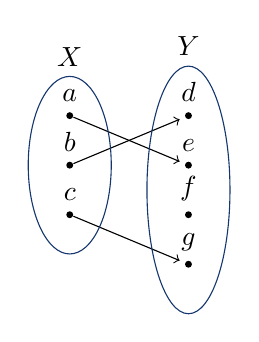
\begin{tikzpicture}
[
  group/.style={ellipse, draw=myblue, minimum height=50pt, minimum width=30pt, label=above:#1},
  my dot/.style={circle, fill, minimum width=2.5pt, label=above:#1, inner sep=0pt}
]
\node (a) [my dot=$a$] {};
\node (b) [below=15pt of a, my dot=$b$] {};
\node (c) [below=15pt of b, my dot=$c$] {};

\node (d) [right=40pt of a, my dot=$d$] {};
\node (e) [right=40pt of b, my dot=$e$] {};
\node (f) [right=40pt of c, my dot=$f$] {};
\node (g) [below=15pt of f, my dot=$g$] {};

\foreach \i/\j in {a/e,b/d,c/g}
  \draw [->, shorten >=2pt] (\i) -- (\j);
\node [fit=(a) (b) (c), group=$X$] {};
\node [fit=(d) (e) (f) (g), group=$Y$] {};
\end{tikzpicture}
%\newpage

\emph{Surjektivität:}\\
$\forall y\in Y\exists x\in X:f(x)=y$\\
Jedes $y\in Y$ wird mindestens einmal getroffen:

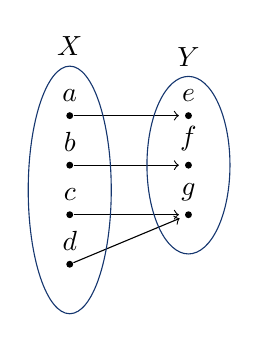
\begin{tikzpicture}
[
  group/.style={ellipse, draw=myblue, minimum height=50pt, minimum width=30pt, label=above:#1},
  my dot/.style={circle, fill, minimum width=2.5pt, label=above:#1, inner sep=0pt}
]
\node (a) [my dot=$a$] {};
\node (b) [below=15pt of a, my dot=$b$] {};
\node (c) [below=15pt of b, my dot=$c$] {};
\node (d) [below=15pt of c, my dot=$d$] {};

\node (e) [right=40pt of a, my dot=$e$] {};
\node (f) [right=40pt of b, my dot=$f$] {};
\node (g) [right=40pt of c, my dot=$g$] {};

\foreach \i/\j in {a/e,b/f,c/g,d/g}
  \draw [->, shorten >=2pt] (\i) -- (\j);
\node [fit=(a) (b) (c) (d), group=$X$] {};
\node [fit=(e) (f) (g), group=$Y$] {};
\end{tikzpicture}

\emph{Bijektivität:}\\
Jedem $x\in X$ wird genau ein $y\in Y$ zugeordnet und jedem $y\in Y$ genau ein $x\in X$:

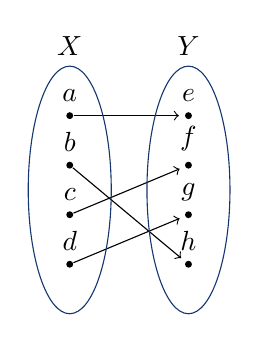
\begin{tikzpicture}
[
  group/.style={ellipse, draw=myblue, minimum height=50pt, minimum width=30pt, label=above:#1},
  my dot/.style={circle, fill, minimum width=2.5pt, label=above:#1, inner sep=0pt}
]
\node (a) [my dot=$a$] {};
\node (b) [below=15pt of a, my dot=$b$] {};
\node (c) [below=15pt of b, my dot=$c$] {};
\node (d) [below=15pt of c, my dot=$d$] {};

\node (e) [right=40pt of a, my dot=$e$] {};
\node (f) [right=40pt of b, my dot=$f$] {};
\node (g) [right=40pt of c, my dot=$g$] {};
\node (h) [right=40pt of d, my dot=$h$] {};

\foreach \i/\j in {a/e,b/h,d/g,c/f}
  \draw [->, shorten >=2pt] (\i) -- (\j);
\node [fit=(a) (b) (c) (d), group=$X$] {};
\node [fit=(e) (f) (g) (h), group=$Y$] {};
\end{tikzpicture}

\emph{Beispiel für Abbildung}, die injektiv aber nicht surjektiv ist: Sei $f:\mathbb{N}\to\mathbb{N}$. Dann ist $f(n)=n+1$ injektiv, da $f(x)=f(y)\Leftrightarrow x+1=y+1$ gelten muss, was nur gilt, wenn $x=y$. $f$ ist nicht surjektiv da $0$ kein Urbild.
\subsection*{Komposition}
Die \emph{Komposition} (Hintereinanderausführung) zweier Abbildungen $f:A\to B$ und\\
$g:B\to C$ ist $a\mapsto (g\circ f)(a)=g(f(a)),\quad a\in A$

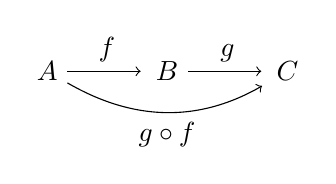
\begin{tikzpicture}
\node at (0,0) (a) {$A$};
\node[right =1cm of a]  (b){$B$};
\node[right =1cm of b]  (c){$C$};
\draw[->, shorten >=2pt] (a) --node[above]{$f$} (b);
\draw[->, shorten >=2pt] (b) --node[above]{$g$} (c);
\draw[->, shorten >=2pt] (a) edge[bend right=30]node[below]{$g\circ f$} (c);
\end{tikzpicture}

Es gilt $(h\circ g)\circ f=h\circ (g\circ f)$. Außerdem gilt:
Die Komposition von injektiven Abbildungen ist injektiv, die von surjektiven Abbildungen ist surjektiv und die von bijektiven Abbildungen ist bijektiv.
\subsection*{Identität, Umkehrabbildung}
Die Abbildung $id_A:A\to A$ mit $id_A(a)=a$ heißt \emph{Identität}.\\
Sei $f:A\to B$ bijektive Abbildung. Dann existiert zu $f$ stets eine Abbildung $g$ mit 
$g\circ f=id_A$ und $f\circ g=id_B$. $g$ heißt die zu $f$ \emph{inverse Abbildung} ($f^{-1}$).
Es gilt $f^{-1}(f(a))=a$ und $f(f^{-1}(b))=b$.
\subsection*{Mächtigkeit von Mengen, Abzählbarkeit}
\emph{Gleichmächtige Mengen:}\\
Seien $M$ und $N$ zwei Mengen. $M$ und $N$ heißen gleichmächtig, wenn es eine bijektive
Abbildung $f:M\to N$ gibt ($M\cong N$).\\
\emph{Endliche Mengen:}\\
Eine Menge $M$ heißt endlich, wenn $M=\emptyset$ oder es für ein $n\in\mathbb{N}$ eine
bijektive Abbildung $b:M\to\mathbb{N}_n$ gibt.\\
\emph{Unendliche Mengen:}\\
Eine Menge $M$ heißt unendlich, wenn $M$ nicht endlich.\\
\emph{Abzählbare Mengen:}\\
Eine Menge $M$ heißt abzählbar, wenn $M$ endlich oder es gibt bijektive
Abbildung $b:M\to\mathbb{N}$.\\
\emph{Abzählbar unendliche Mengen:}\\
Eine Menge $M$ heißt abzählbar unendlich, wenn $M$ abzählbar und $M$ unendlich.\\
\emph{Überabzählbare Mengen:}\\
Eine Menge $M$ heißt überabzählbar, wenn $M$ nicht abzählbar.\\
\emph{Spezielle endliche Mengen:}\\
Sei $n\in\mathbb{N}$. Dann ist $\mathbb{N}_n:=[n]:=\{1,...,n\}$ die Menge der ersten
$n$ natürlichen Zahlen.\\
\emph{Beispiele:}\\
$|\{a,b,c\}|=3=|\{x,y,11\}|$\\
$|\mathbb{N}|=|\mathbb{R}|=|\mathbb{N}\times\mathbb{N}|$
\subsection*{Kardinalität}
Anzahl der Elemente einer Menge. Zwei Mengen haben gleiche Kardinalität, wenn
sie gleichmächtig sind.
\subsection*{Beispielbeweis}
\emph{Zu zeigen:} $|\mathbb{N}|=|\mathbb{N}\times\mathbb{N}|$\\
\emph{Beweis.} Wir betrachten $f:\mathbb{N}\to\mathbb{N}\times\mathbb{N}$ mit
$f(n):=(1,n)$ und $g:\mathbb{N}\times\mathbb{N}\to\mathbb{N}$ mit $g(n,m):=2^n\cdot 3^m$.
Beide sind injektiv, also $\mathbb{N}\cong\mathbb{N}\times\mathbb{N}$, also
$|\mathbb{N}|=|\mathbb{N}\times\mathbb{N}|$.
%\section{Beweistechniken}
\subsection*{Direkter Beweis}
Beim direkten Beweis wird Schritt für Schritt mittels \emph{Wenn, Dann} bewiesen.
\subsection*{Kontraposition}
Da $p\Rightarrow q\equiv \neg q\Rightarrow \neg p$ kann man die Aussage auch mittels Kontraposition beweisen.
\subsection*{Widerspruch}
Beim Widerspruchsbeweis wird Gegenteil angenommen und in einen Widerspruch geführt.
Also muss die ursprüngliche Aussage wahr sein.
\subsection*{Äquivalenzbeweis}
Beweis über zeigen der Hin- und Rückrichtung.
\subsection*{Fallunterscheidung}
Beweis aller möglichen Fälle.
\subsection*{Induktionsbeweis}
Induktionsanfang ($n$ kleinste Zahl):\\
Induktionsbehauptung: Aussage gelte für beliebiges aber festes $n\in \mathbb{N}$ mit $n\geq$ kleinste Zahl.\\
Induktionsschluss ($n \Longrightarrow n+1$): Zu zeigen ist also $n+1$ einsetzen $\Rightarrow$ Aussage gilt auch,
\emph{mit Benutzung von Induktionsbehauptung}.
%\subsection*{VI an Rekursiver Funktion} 
%\section{Graphentheorie}
\subsection*{Gerichteter Graph}
$G=(V,E)$ wobei $V$ Menge aller Knoten z.B. $V=\{v_0,v_1,v_2,\dots,v_n\}$ und $E\subseteq V\times V$ Menge aller Kanten mit $e=(v,u)$. Hierbei steht $v$ für den Startknoten von $e$ und $u$ ist Endknoten von $e$.\\
\emph{Hinweis:}\\
Ist die Kantenmenge $E$ symmetrisch ($(u,v)\in E\wedge (v,u)\in E$) sprechen wir von einem ungerichteten Graphen. In solchen werden keine Schlingen betrachtet.
\subsection*{Adjazente Knoten}
Zwei Knoten, die in einem Graphen durch eine Kante verbunden sind, heißen \emph{adjazent} oder \emph{benachbart}.
\subsection*{Endlicher Graph}
Ein Graph $G$ heißt endlich, wenn die Knotenmenge $V$ endlich ist.
\subsection*{Nullgraph (vollst. unverbunden)}
$G=(V,\emptyset)\Rightarrow$ ohne Kanten
\subsection*{Vollständiger Graph}
$G=(V,V\times V)$ ist vollständig (heißt auch $K_n$ wegen $n$ Knoten) und hat Maximalzahl von $n^2$ Kanten $\Rightarrow$ gerichtet und mit Schlingen. Der Ungerichtete $K_n$ hat $\frac{n\cdot (n-1)}{2}$ Kanten, wobei $n$ die Zahl der Knoten ist.\\
\emph{Beispiel:}\\
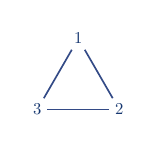
\begin{tikzpicture}[scale=.60,transform shape]
\graph [simple,nodes={myblue}, edges={myblue!80, semithick}] {subgraph K_n [n=3, clockwise];};
\end{tikzpicture}
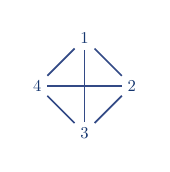
\begin{tikzpicture}[scale=.60,transform shape]
\graph [simple,nodes={myblue}, edges={myblue!80, semithick}] {subgraph K_n [n=4, clockwise];};
\end{tikzpicture}
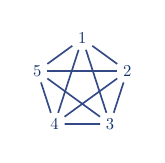
\begin{tikzpicture}[scale=.60,transform shape]
\graph [simple,nodes={myblue}, edges={myblue!80, semithick}] {subgraph K_n [n=5, clockwise];};
\end{tikzpicture}
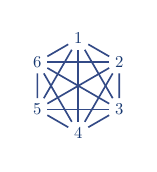
\begin{tikzpicture}[scale=.60,transform shape]
\graph [simple,nodes={myblue}, edges={myblue!80, semithick}] {subgraph K_n [n=6, clockwise];};
\end{tikzpicture}
\subsection*{Ungerichteter Graph}
Ein Graph $G=(V,E)$ ist ungerichtet $\Leftrightarrow E$ ist symmetrisch $\Leftrightarrow (u,v)\in E\wedge (v,u)\in E$. Da hier die Kanten ungerichtet, kann Mengenschreibweise verwendet werden.
\subsection*{Schlinge}
Kante mit gleichem Start- und Endknoten. Wird bei ungerichteten Graphen nicht betrachtet.
\subsection*{Bipartite Graphen}
Ein ungerichteter Graph ist bipartit, wenn die Knotenmenge $V$ in zwei disjunkte Teilmengen $U,W$ zerlegbar ist, sodass alle Kanten $e\in E$ einen Endpunkt in $U$ und einen anderen in $W$ haben.\\
\emph{Beispiel:}\\
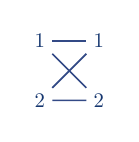
\begin{tikzpicture}[scale=.75,transform shape]
\graph [simple,nodes={myblue}, edges={myblue!80, semithick}] {subgraph K_nm [n=2,m=2];};
\end{tikzpicture}
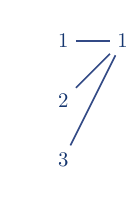
\begin{tikzpicture}[scale=.75,transform shape]
\hspace{.3cm}
\graph [simple,nodes={myblue}, edges={myblue!80, semithick}] {subgraph K_nm [n=3,m=1];};
\end{tikzpicture}
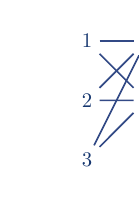
\begin{tikzpicture}[scale=.75,transform shape]
\hspace{.6cm}
\graph [simple,nodes={myblue}, edges={myblue!80, semithick}] {subgraph K_nm [n=3,m=2];};
\end{tikzpicture}
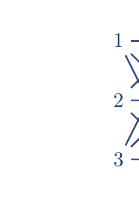
\begin{tikzpicture}[scale=.75,transform shape]
\hspace{1cm}
\graph [simple,nodes={myblue}, edges={myblue!80, semithick}] {subgraph K_nm [n=3,m=3];};
\end{tikzpicture}
\subsection*{Eulersche Graphen}
$G$ heißt eulerscher Graph, falls es in $G$ einen geschlossenen Weg gibt, der jede Kante von $G$ enthält.\\
$G$ ist eulerscher Graph $\Leftrightarrow$ jede Ecke von $G$ hat geraden Grad und $G$ ist zusammenhängend.
\subsection*{Untergraph}
Seien $G=(V_G,E_G)$, $H=(V_H,E_H)$ zwei Graphen. $H$ heißt Teilgraph von $G$, wenn $V_H\subseteq V_G$ und $E_H\subseteq E_G$
(wenn also jede Kante von $H$ auch zu $G$ gehört.)\\
\emph{Hinweis:}\\
Der Nullgraph $O_n$ ist Teilgraph jedes Graphen mit $n$ Knoten. Außerdem ist jeder Graph Teilgraph des vollständigen Graphen $K_n$.
\subsection*{Induzierte Teilgraphen}
Sei $G=(V,E)$ ein Graph. Ist $V'\subseteq V$ eine Teilmenge der Knotenmenge $V$ von $G$, dann ist der Untergraph oder
der durch $V'$ induzierte Teilgraph von $G$ der Graph $G[V']=(V',E')$ mit $E'=\{(u,v)\mid u,v\in V'\wedge (u,v)\in E\}$\\
\emph{Beispiel:}\\
Ist $G$ ein Graph hat $G[\{2,3,4\}]$ nur die Knoten $2$, $3$ und $4$ und die entsprechenden Kanten.
\subsection*{Grad eines Knoten}
Der Ausgrad von $v$ ist die Zahl der Kanten, die $v$ als Startknoten besitzen.
Der Ingrad von $v$ ist die Zahl der Kanten, die in $v$ enden.
Ist $G$ ungerichtet stimmen Ausgrad von $v$ und Ingrad von $v$ überein und wird Grad von $v$ genannt.\\
\emph{Hinweis:}\\
Sei $G=(V,E)$ gerichteter Graph, dann gilt $\sum_{v\in V} indeg(v)=\sum_{v\in V} outdeg(v)=|E|$.
Ist $G$ ungerichtet, dann gilt $\sum_{v\in V} deg(v)=2\cdot |E|$.
\subsection*{Wege}
Ein Weg von den Knoten $u$ nach $v$ ist eine Folge benachbarter Knoten. Die Länge
eines Weges ist die Anzahl der Kanten. Ein Weg der Länge $0$ wird als trivialer Weg bezeichnet und besteht nur aus einem Knoten.\\
\emph{Hinweis:}\\
Ein Weg heißt geschlossen, wenn seine beiden Endknoten gleich sind.
\subsection*{Graphzusammenhang}
Knoten $u$ und $v$ eines ungerichteten Graphen heißen zuammenhängend, wenn es
einen Weg in $G$ von $u$ nach $v$ gibt.
\subsection*{Zusammenhangskomponente}
Ein Graph $G$ heißt zusammenhängend wenn jedes Knotenpaar aus $G$ zusammenhängend ist.\\
\emph{Hinweis:}\\
Die Äquivalenzklassen (zusammenhängende Teilgraphen) einer Zusammenhangsrelation $Z$ über einem ungerichteten Graphen $G$ heißen Zusammenhangskomponenten (ZK) von $G$.
\subsection*{Pfade, Kreise}
Als \emph{Pfad} werden Wege in einem Graphen bezeichnet, bei denen keine Kante zweimal durchlaufen wird.
Ein geschlossener Pfad heißt \emph{Kreis}. Bei einem \emph{einfachen Pfad} wird kein Knoten mehrfach durchlaufen.
Ein geschlossener Pfad, der mit Ausnahme seines Ausgangspunktes einfach ist, heißt \emph{einfacher Kreis}.
Ein einfacher Kreis durch sämtliche Knoten des Graphen, heißt \emph{Hamiltonscher Kreis}.
\subsection*{Hamiltonscher Kreis}
Kann der Zusammenhang eines Graphen $G$ durch die Entnahme eines einzigen Knotens (und
sämtlicher mit diesem Knoten benachbarter Kanten) zerstört werden, dann besitzt $G$ keinen
Hamiltonschen Kreis.
\subsection*{Isomorphe Graphen}
Zwei Graphen heißen isomorph zueinander, wenn sie strukturell gleich sind.\\
\emph{Beispiel:}\\
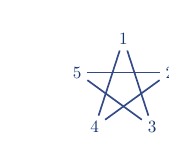
\begin{tikzpicture}[scale=.62,transform shape]
\hspace{.5cm}
\graph [simple,nodes={myblue}, edges={myblue!80, semithick}] {subgraph K_n [n=5, clockwise];
1 -!- 2;
2 -!- 3;
3 -!- 4;
4 -!- 5;
5 -!- 1;
};
\end{tikzpicture}
\begin{tikzpicture}[scale=.62,transform shape]
\hspace{.75cm}
\graph [simple,nodes={myblue}, edges={myblue!80, semithick}] {subgraph K_n [n=5, clockwise];
1 -!- 4;
1 -!- 3;
5 -!- 2;
5 -!- 3;
4 -!- 2;
};
\end{tikzpicture}

\begin{tabular}{c|c|c|c|c|c}
$v$ & $1$ & $2$ & $3$ & $4$ & $5$ \\ 
$\phi (v)$ & $1$ & $4$ & $2$ & $5$ & $3$ \\
\end{tabular}
\subsection*{Komplementäre Graphen}
Sei $G=(V,E)$ ein Graph. Dann ist $\bar{G}=(V,(V\times V)\setminus E)$ der Komplementärgraph von $G$.\\
\emph{Hinweis:}\\
Ein Graph heißt selbstkomplementär wenn $G$ und $\bar{G}$ isomorph sind.
%\subsection*{Wälder, Bäume}
%Ein Graph heißt \emph{zyklenfrei}, wenn er keinen geschlossenen Weg der Länge $\geq 1$ besitzt.
%Ein ungerichteter Graph heißt \emph{Wald}, wenn er zyklenfrei ist.
%Ein ungerichteter Graph heißt Baum, wenn er zyklenfrei und zusammenhängend ist.
%Ein wesentliches Charakteristikum von Bäumen ist die Tatsache, dass jedes Paar von
%Knoten in einem Baum durch genau einen Weg verbunden ist.
%Werden in einem Baum Kanten gestrichen, dann entsteht ein Wald
%Die Knoten eines Baumes vom Grad 1 werden \emph{Blätter} genannt, die Knoten vom Grad
%größer als 1 heißen \emph{innere Knoten}.
%Ist $G$ ein zusammenhängender Graph mit $n$ Knoten und $n-1$ Kanten, dann ist $G$ ein
%Baum.
%Als \emph{Tiefe eines Knotens} von $T$ wird sein Abstand von der Wurzel bezeichnet.
%Die Tiefe von $T$ ist die größte Knotentiefe.  Alle Knoten der gleichen Tiefe bilden ein \emph{Knotenniveau}.
%Als \emph{Kinder eines Knotens} $v$ von $T$ werden sämtliche Knoten bezeichnet, die zu $v$
%benachbart sind und deren Tiefe die von $v$ um eins übersteigt. $v$ heißt \emph{Vater} seiner Kinder.
%\subsection*{Vollst. binärer Baum}
%Ein \emph{vollständiger binärer Baum} ist ein binärer Baum, bei dem jeder innere Knoten
%genau zwei Kinder hat.
%Sei $T$ ein vollständiger binärer Baum mit $k$ inneren Knoten.
%$T$ hat $k+1$ Blätter und insgesamt $2k+1$ Knoten.
%Sei $d$ die Tiefe von $T$, dann besitzt $T$ insgesamt $\sum_{i=0}^d 2^i=2^{d+1}-1$ Knoten.

%\section{Graphenalgorithmen}
\subsection*{Kantenlänge}
Jeder Kante wird eine reelle Zahl zugeordnet, die wir als Länge dieser Kante bezeichnen.
Man spricht dann von einem Graphen mit bewerteten Kanten
\subsection*{Algorithmus von Dijkstra}
Dient der \emph{Bestimmung kürzester Wege} von einem fest vorgegebenen Knoten zu allen anderen Knoten
in einem schlichten, zusammenhängenden, gerichteten Graphen mit endlicher Knotenmenge und nicht-negativ bewerteten Kanten
und liefert einen Weg mit einer minimalen Gesamtlänge.\\
\emph{Algorithmus}\\
Schreibe Tabelle mit Knoten, Entfernung, Vorgänger, OK\\
Setze alle Entf. auf $\infty$ außer $Start=0$\\
Setze Vorg. von $Start=Start$\\
Setze alle $OK=f$\\
Starte Algorithmus:\\
Wiederhole:\\
	Suche unter den Entfernungen die kleinste$=j$, die $OK=f$ ($\Rightarrow$ beim Start also $Start$ selbst)\\
		Setze $j=t$\\
		Suche alle Nachbarknoten $k$ von $j$, die noch nicht $t$ sind.\\
		Wenn die Entfernung größer als $j+k$ setze neue Entf. und setze neuen Vorgänger.\\	
Solange bis noch Knoten mit $OK=f$
\subsection*{Flussprobleme}
Modellierung von Transport von Gütern (Strom, Container etc.) entlang der Kanten.\\
$c(e_{ij})=c_{ij}$ ist Kapazität einer Kante. $v_iv_j=e_{ij}$ ist die Menge eines Gutes,
die entlang der Kante transportiert werden kann.
\subsection*{Fluss}
Ein Fluss in $G$ von der Quelle $q=v_1$ zur Senke $s=v_n$ ist eine Funktion $f$, die jeder
Kante $e_{ij}\in E$ eine nicht-negative rationale Zahl zuordnet.
\subsection*{Schnitt}
Seien $X,Y$ bel. Untermengen von Knoten eines Graphen $G$. Dann ist\\
$A(X,Y)$ die Menge der Kanten, die Knoten aus $X$ mit Knoten $Y$ verbinden.\\
$A^+(X,Y)$ ist die Menge der Kanten, ausgehend von Knoten aus $X$, die Knoten aus $Y$
verbinden.\\
$A^-(X,Y)$ ist die Menge der Kanten, ausgehend von Knoten aus $Y$, die Knoten aus $X$
verbinden.\\
Sei $g$ eine Funktion, die den Kanten eines Graphen $G$ nicht-negative Zahlen zuordnet, dann
gilt $g(X,Y)=\sum_{e\in A^+(X,Y)}g(e)$.\\
Ein \emph{Schnitt} ist eine Menge von Kanten $A(X,\bar{X})$ mit $q\in X$ und $s\in\bar{X}$.\\
\emph{Beispiel:}\\
Wähle $X=\{q=v_1,...\}$ und $\bar{X}=\{...,s=v_n\}$ mit $...$ beliebig. Dann ist $A(X,\bar{X})=\{e_{ij},e_{...}\}$ die Menge der Kanten zwischen $X$ und $\bar{X}$.\\
$A^+(X,\bar{X})=\{e_{ij},e_{...}\}$ die Menge der Kanten aus $X$.\\
$A^-(X,\bar{X})=\{e_{ij},e_{...}\}$ die Menge der Kanten in $X$ hinein.\\
Der \emph{Fluss} von den Knoten in $X$ zu den Knoten in $\bar{X}$ ist dann:\\
$\sum_{e_{ij}\in A^+(X,Y)}f(e_{ij})-\sum_{e_{ij}\in A^-(X,Y)}f(e_{ij})$ Hierbei steht $f(e_{ij})$ für den Fluss, also der hinteren Zahl im Tupel $(x,y)$ an der Kantenbeschriftung.\\
Die \emph{Kapazität} bestimmt man aus der vorderen Zahl jenen Tupels wie folgt:\\
$c(X,\bar{X})=\sum_{e_{ij}\in A^+(X,Y)}c(e_{ij})$\\
\emph{Hinweis:}\\
Es gibt $2^n$ mögliche Schnitte wenn $n$ die Anzahl der inneren Knoten ist.
\subsection*{Maximaler Fluss}
Ein Fluss $f$, dessen Wert $d$ maximal ist, heißt \emph{maximaler Fluss}.\\
Ein Fluss dessen Wert $\min\{c(X,\bar{X})\}$ entspricht, ist maximal.
\subsection*{Vergrößernder Weg}
Ein ungerichteter Weg von $q$ nach $s$ heißt \emph{vergrößernd}, wenn
für jede Kante $e_{ij}$ auf dem Weg ihrer Richtung gilt: $f(e_{ij})<c(e_{ij})$
(Vorwärtskante) bzw. $f(e_{ij})>0$ (Rückwärtskante).
\subsection*{Algorithmus von Ford und Fulkerson}
Initialsiere alle Flüsse mit 0.\\
Wiederhole:\\
	Suche guten Fluss, der optimal wird und schreibe Tabelle:\\
	$1) q(\bot,\infty) v_x(+q,Anzahl), ... , s(+v_{...},Anzahl)$\\
	Trage Fluss nach Komma ein.\\
Bis:\\
Es gibt keinen weiteren vergrößernden Fluss.\\
Antwort: max. Fluss mit $d=...$\\
\emph{Hinweis:} Nur soviel durchschicken wie benötigt und evtl. größte Flüsse zuerst.
%\section{Algebraische Strukturen}
\subsection*{Monoid}
Ein Monoid ist ein Tupel $(M,*,e)$ bestehend aus einer Menge $M$, einer zweistelligen
Verknüpfung $*:M\times M\to M,\quad (a,b)\mapsto a*b$ und einem neutralem Element $e\in M$.
Außerdem muss gelten:\\
Assoziativität:\\
(M1) $\forall a,b,c\in M:(a*b)*c=a*(b*c)$\\
neutrales Element:\\
(M2) $\forall a\in M:e*a=a*e=a$\\
\emph{Beispiel:}\\
$(\mathbb{N}_0,+,0)$ ist Monoid\\
$(\mathbb{N},\cdot,1)$ ist Monoid
\subsection*{Gruppe}
Eine Gruppe ist ein Tupel $(G,*,e,a^{-1})$ bestehend aus einer Menge $G$, einer zweistelligen Verknüpfung $*:G\times G\to G,\quad (a,b)\mapsto a*b$, einem neutralem Element $e\in G$ und einem inversen Element $a^{-1}\in G$.
Außerdem muss gelten:\\
Abgeschlossenheit:\\
(G1) $\forall a,b\in G:(a*b)\in G$\\
Assoziativität:\\
(G2) $\forall a,b,c\in G:(a*b)*c=a*(b*c)$\\
neutrales Element:\\
(G3) $\forall a\in G:e*a=a*e=a$\\
inverses Element:\\
(G4) $\forall a\in G\exists a^{-1}\in G:a*a^{-1}=a^{-1}*a=e$\\
Für abelsche Gruppe:\\
Kommutativität:\\
(G5) $\forall a,b\in G:a*b=b*a$\\
\emph{Beispiel:}\\
$(\mathbb{Z},+,0,-a)$ ist Gruppe\\
$(\mathbb{Q}\setminus\{0\},\cdot,1,\frac{1}{a})$ ist Gruppe
\subsection*{Körper}
Ein Körper ist ein Tupel $(K,+,\cdot)$, bestehend aus einer Menge $K$ und zwei 
zweistelligen Operationen $+$ und $\cdot$ auf $K$.\\
Es muss gelten:\\
(K1) $(K,+)$ ist abelsche Gruppe mit neutralem Element $0$.\\
(K2) $(K\setminus \{0\},\cdot)$ ist abelsche Gruppe mit neutralem Element $1$.\\
(K3) Distributivität:\\
$\forall a,b,c\in K:a\cdot (b+c)=a\cdot b+a\cdot c$\\
\emph{Beispiel:}\\
$(\mathbb{Q},+,\cdot)$ ist Körper\\
$(\mathbb{R},+,\cdot)$ ist Körper
%\subsection*{Schaltfunktionen}
%\subsection*{Boolsche Algebra}
%\section{Formelsammlung}
\subsection*{Binomische Formeln}
$(a+b)^2 = a^2 + 2ab + b^2$\\
$(a-b)^2 = a^2 - 2ab + b^2$\\
$(a+b) \cdot (a-b) = a^2 - b^2$\\
$(a \pm b)^3 = a^3 \pm 3 a^2 b + 3 a b^2 \pm b^3$\\
$(a \pm b)^4 = a^4 \pm 4 a^3 b + 6 a^2 b^2 \pm 4 a b^3 + b^4$\\
$(a \pm b)^5 = a^5 \pm 5 a^4 b + 10 a^3 b^2 \pm 10 a^2 b^3 + 5 a b^4 \pm b^5$
\subsection*{Potenzgesetze}
$a^{-n}=\frac{1}{a^n}$\\
$a^m\cdot a^n=a^{m+n}$\\
$\frac{a^m}{a^n}=a^{m-n}$\\
$(a^m)^n=a^{m\cdot n}$\\
$a^n\cdot b^n=(a\cdot b)^n$\\
$\frac{a^n}{b^n}=(\frac{a}{b})^n$
\subsection*{Wurzelgesetze}
$\sqrt[n]{a}=a^{\frac{1}{n}}$\\
$\sqrt[n]{a^m}=(\sqrt[n]{a})^m=a^{\frac{m}{n}}$\\
$\sqrt[n]{a}\cdot\sqrt[n]{b}=\sqrt[n]{a\cdot b}$\\
$\frac{\sqrt[n]{a}}{\sqrt[n]{b}}=\sqrt[n]{\frac{a}{b}}$\\
$\sqrt[n]{\sqrt[m]{a}}=\sqrt[{n\cdot m}]{a}$
\subsection*{Summeneigenschaften}
%$\sum_{i=1}^n c=n\cdot c$\\
%$\sum_{i=m}^n c=(n-m+1)\cdot c$\\
$\sum_{i=m}^n c\cdot a_i=c\cdot \sum_{i=m}^n a_i$\\
$\sum_{i=m}^n (a_i+b_i)=\sum_{i=m}^n a_i + \sum_{i=m}^n b_i$
\subsection*{Summenformeln}
Gaußsche Summenformel:\\
$\sum_{i=1}^n i=\frac{n(n+1)}{2}$\\
Geometrische Reihe:\\
$\sum_{i=1}^n q^i=\frac{1-q^{n+1}}{1-q}$\\
Potenzsummen:\\
$\sum_{i=1}^n i^2=\frac{n(n+1)(2n+1)}{6}$\\
$\sum_{i=1}^n i^3=\frac{n^2(n+1)^2}{4}$
\subsection*{Potenzmengen}
  $  \mathcal P(\emptyset) = \{ \emptyset \}\mathcal P(\{ a \}) = \bigl\{ \emptyset, \{ a \} \bigr\}\\
    \mathcal P(\{ a, b \}) = \bigl\{ \emptyset, \{ a \}, \{ b \}, \{ a, b \} \bigr\}\\
    \mathcal P(\{ a, b, c \}) = \bigl\{ \emptyset, \{ a \}, \{ b \}, \{ c \}, \{ a, b \}, \{ a, c \}, \{ b, c \}, \{ a, b, c \} \bigr\}\\
    \mathcal P(\mathcal P(\emptyset)) = \bigl\{ \emptyset, \{\emptyset\}\bigr\}\\
    \mathcal P(\mathcal P(\{a\})) = \bigl\{ \emptyset, \{\emptyset\} , \{\{a\}\} , \{\emptyset , \{a\}\} \bigr\}$
\end{multicols*}



\end{document}